\documentclass[11pt,letterpaper,titlepage,en-US]{article}

\usepackage{basicstyle}
\usepackage{homework}
%
% Homework Details
%   - Title
%   - Due date
%   - Class
%   - Section/Time
%   - Instructor
%   - Author
%

\newcommand{\hmwkTitle}{Homework\ \#3 }
\DTMsavetimestamp{DueDate}{2016-11-09T23:59:59-06:00}
\newcommand{\hmwkClass}{CS 6363.005}
\newcommand{\hmwkClassName}{Design and Analysis of Computer Algorithms}
\newcommand{\hmwkClassInstructor}{Instructor: Benjamin Raichel}
\newcommand{\hmwkAuthorName}{Hanlin He}
\newcommand{\hmwkAuthorNetID}{hxh160630}
\newcommand{\hmwkAuthorUTDEmail}{\href{mailto:hanlin.he@utdallas.edu}{hanlin.he@utdallas.edu}}


%
% Title Page
%

\title{
    \vspace{2in}
    \textmd{\textbf{\hmwkClassName \\\hmwkClass:\ \hmwkTitle}}\\
    \normalsize\vspace{0.1in}\small{Due\ on\ \DTMusedate{DueDate}\ at \DTMusetime{DueDate} }\\
    \vspace{0.1in}\large{\textit{\hmwkClassInstructor}}
    \vspace{3in}
}

\author{\textbf{\hmwkAuthorName\ \footnotesize{(\hmwkAuthorNetID)}} \\  \hmwkAuthorUTDEmail}
\date{}
\makeindex

\begin{document}
\maketitle

\pagenumbering{Roman}

\tableofcontents

\pagebreak
\pagenumbering{arabic}

\begin{homeworkProblem}[Fractional Jewelry Collection]

\begin{homeworkSubProblem}[Algorithm Description]

Each time, take the whole jewelry with the largest $V[i]/S[i]$ value,
until the bag's space is insufficient for the next whole jewelry.
And then, cut the next largest $V[i]/S[i]$ value jewelry to fit
the remaining bag's space and take it. As a result, the total value
in the bag will be optimal.

\end{homeworkSubProblem}

\begin{homeworkSubProblem}[Proof of Correctness]

\begin{proof}
Divide the bag into $b$ units with each unit size of $1$.

Assume each unit is the minimal size to fill,
and each time we cut a piece of one jewelry of a unit size
to put in the bag. Putting a whole jewelry into the bag equals
to putting all its pieces with unit size into the bag.

Based on the description of part a, 
each time we put a piece into the bag, its value
must be the largest among the remaining jewelry pieces,
since the pieces with bigger value has already been taken.

Assume there is a optimal solution other than the greedy solution
described in part a. Then, there is a unit size jewelry piece different
in the choosing order,
and its value should be larger than the piece chosen in the greedy
solution. However, all jewelry with larger value has already been taken
in the greedy solution. Thus, it cause a contradiction.

In conclusion, the greedy solution described in part a is optimal.
\end{proof}

\end{homeworkSubProblem}

\end{homeworkProblem}


\begin{homeworkProblem}[Counting Paths]

For any node $s$, let $PC(s,t)$ denote the paths count
from $s$ to $t$. If $G$ is a dag, this function satisfies
the recurrence:
\begin{equation}
PC(s,t) = \left\{
    \begin{array}{ll}
        1 & \text{ if } s = t \\
        0 & \text{ if $s$ is a sink. } \\
        \sum_{s \rightarrow v} PC(v,t) & \text{ otherwise. }\\
    \end{array}
    \right.
\end{equation}
where $\sum_{s \rightarrow v} PC(v,t)$ is the sum of $PC(v,t)$
for all edges $s \rightarrow v$. In particular, if $s$
is a sink but not equal to $t$, then $PC(s,t) = 0$,
since there is no path from $s$ to $t$.

The dependency graph for this recurrence is the input graph
$G$ itself: subproblem $PC(u,t)$ depends on subproblem
$PC(v,t)$ if and only if $u \rightarrow v$ is en edge in $G$.
Thus we can evaluate this recursive function in \bigO{V + E}
time by performing a depth-first-search of $G$, starting at $s$.

The algorithm is shown is \cref{counting_path},
in which $PC[s]$ denote the paths count from $s$ to $t$.

\begin{algorithm}[H]
\caption{Counting Paths Algorithm}\label{counting_path}
\begin{algorithmic}[1]
    \Procedure{CountingPaths}{$s,t$}
        \If{$s = t$}
            \Return $1$
        \EndIf
        \If{$PC[s]$ is undefined}
            \State $PC[s] = 0$
            \Comment{Initially, whether $t$ is reachable from $s$ is unknown.}
            \For{each edge $s \rightarrow v$}
            \Comment{If $s$ is a sink, this For-Loop is skipped.}
                \State $PC[s] = PC[s] + \ProcedureName{CountingPaths}{v,t}$
            \EndFor
        \EndIf
    \Return $PC[s]$
    \EndProcedure
\end{algorithmic}
\end{algorithm}
\end{homeworkProblem}


\begin{homeworkProblem}

\begin{homeworkSubProblem}
    The DFS\&BFS from vertex $a$ are shown in \cref{1.a} and \cref{1.b}.

    \begin{figure}[H]
        \caption{DFS\&BFS for First Graph}\label{1.a}
        \centering
        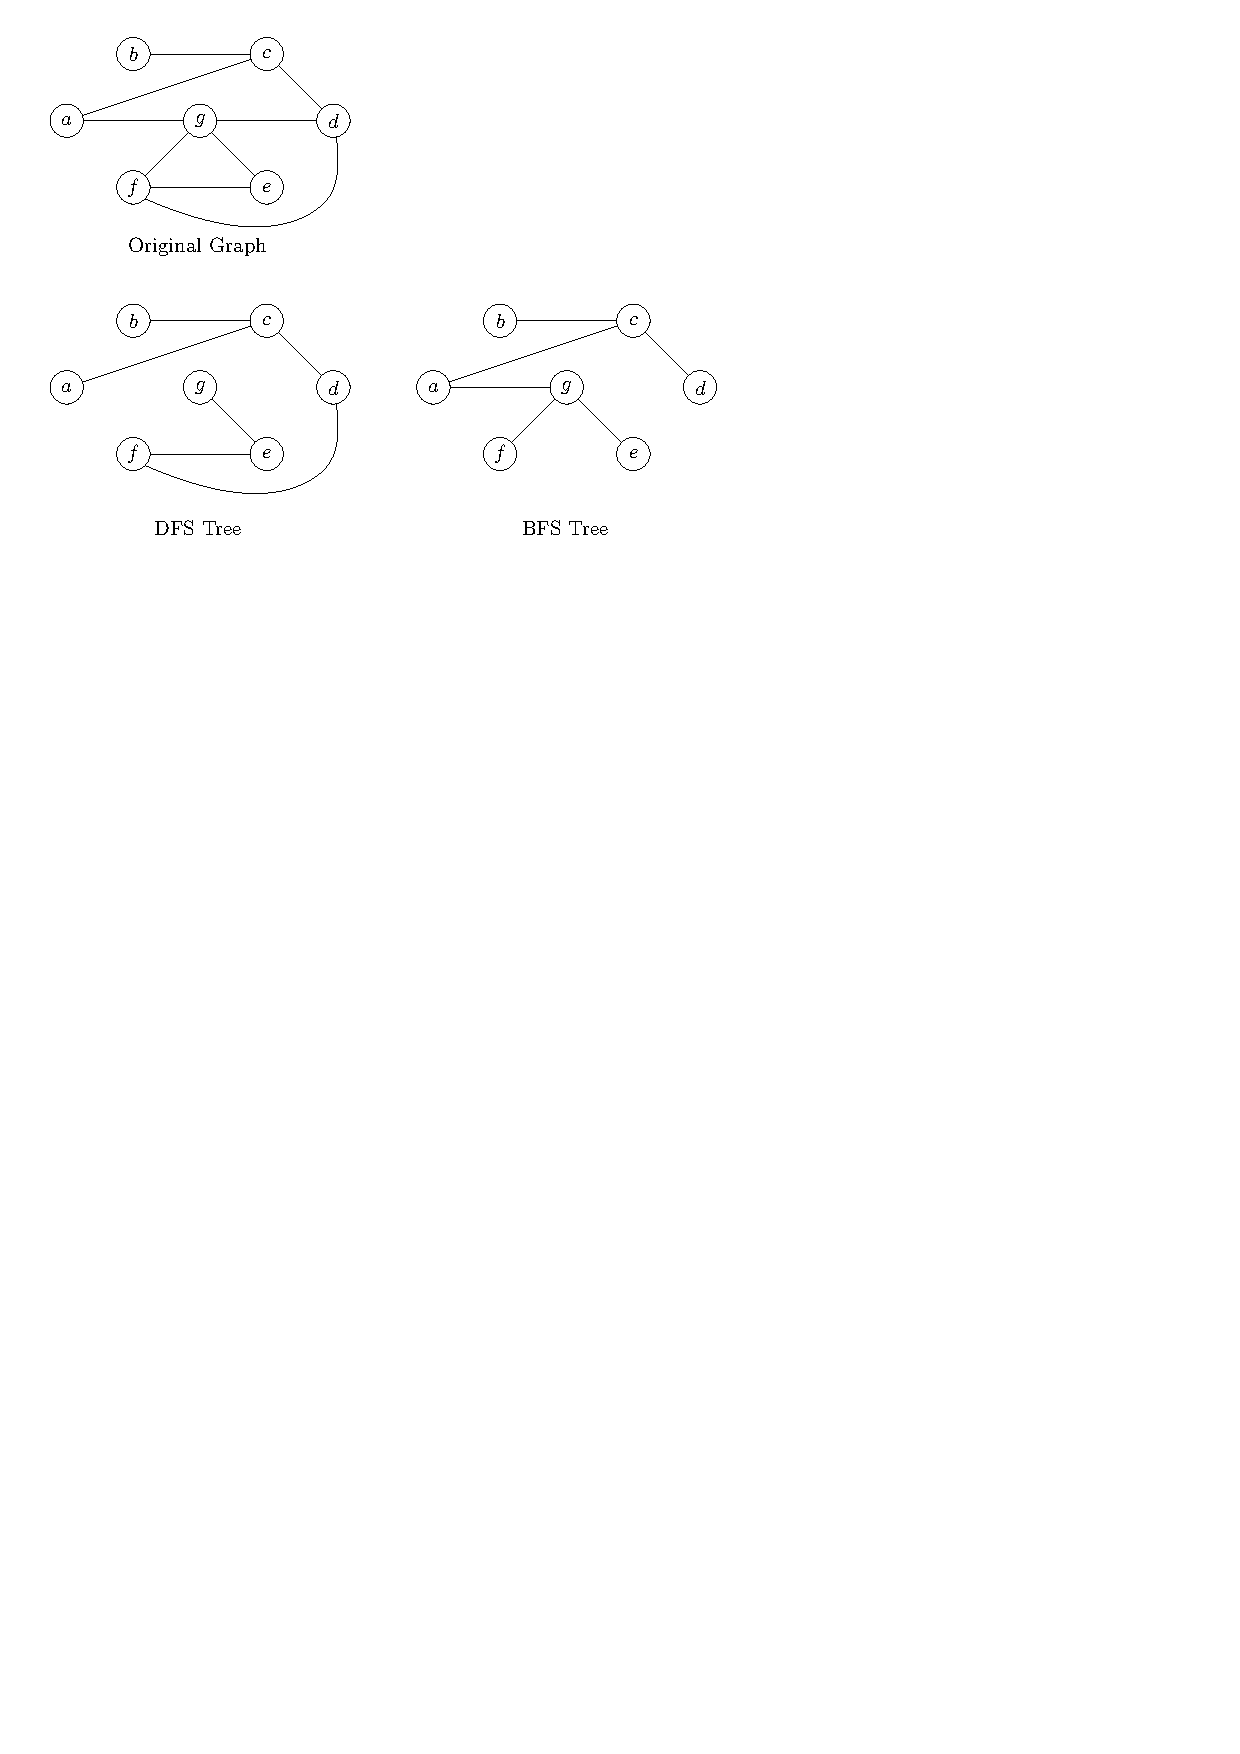
\includegraphics[width=.8\textwidth]{running1a}
    \end{figure}

    \begin{figure}[H]
        \caption{DFS\&BFS for Second Graph}\label{1.b}
        \centering
        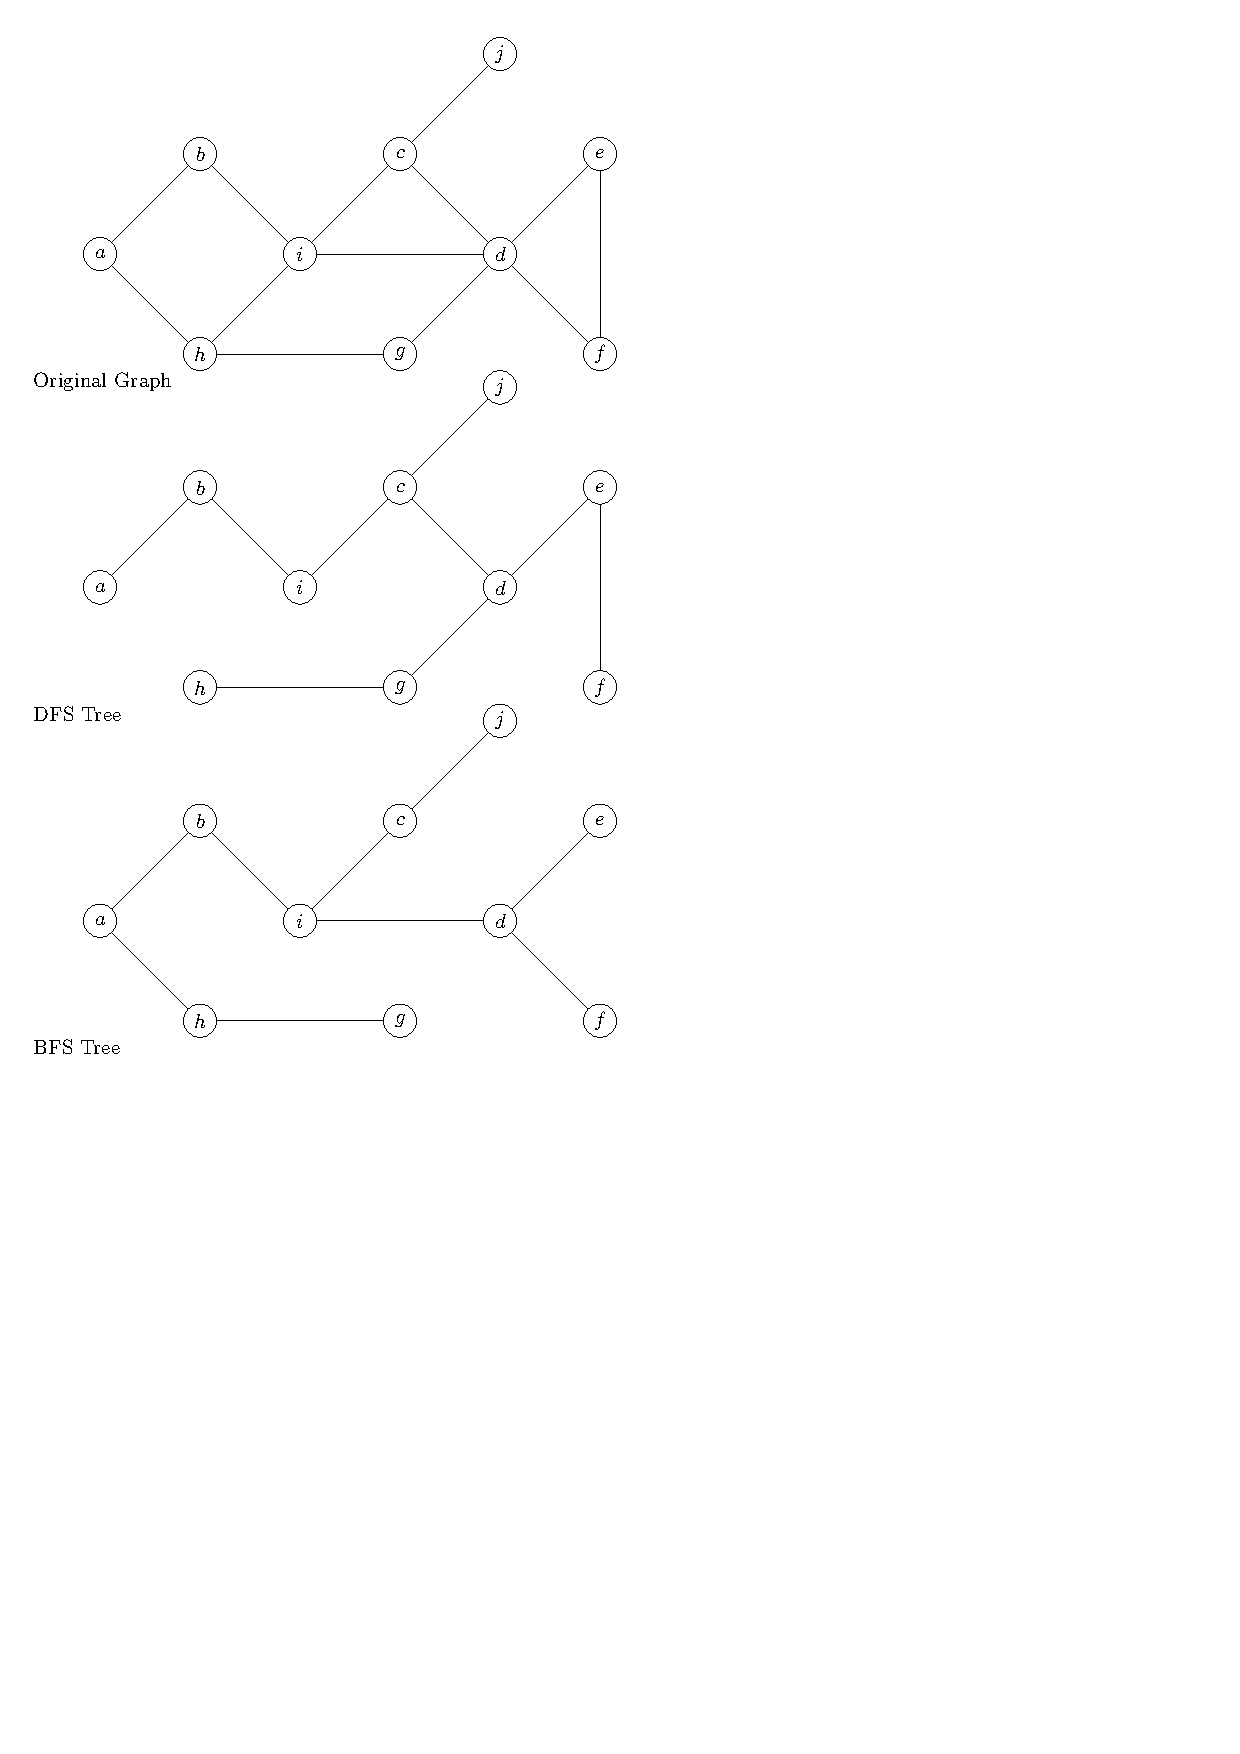
\includegraphics[width=.65\textwidth]{running1b}
    \end{figure}
\end{homeworkSubProblem}

\pagebreak
\begin{homeworkSubProblem}
    The DFS\&BFS from vertex $a$ are shown in \cref{2.a} and \cref{2.b}.

    \begin{figure}[H]
        \caption{Topological Order for First Graph}\label{2.a}
        \centering
        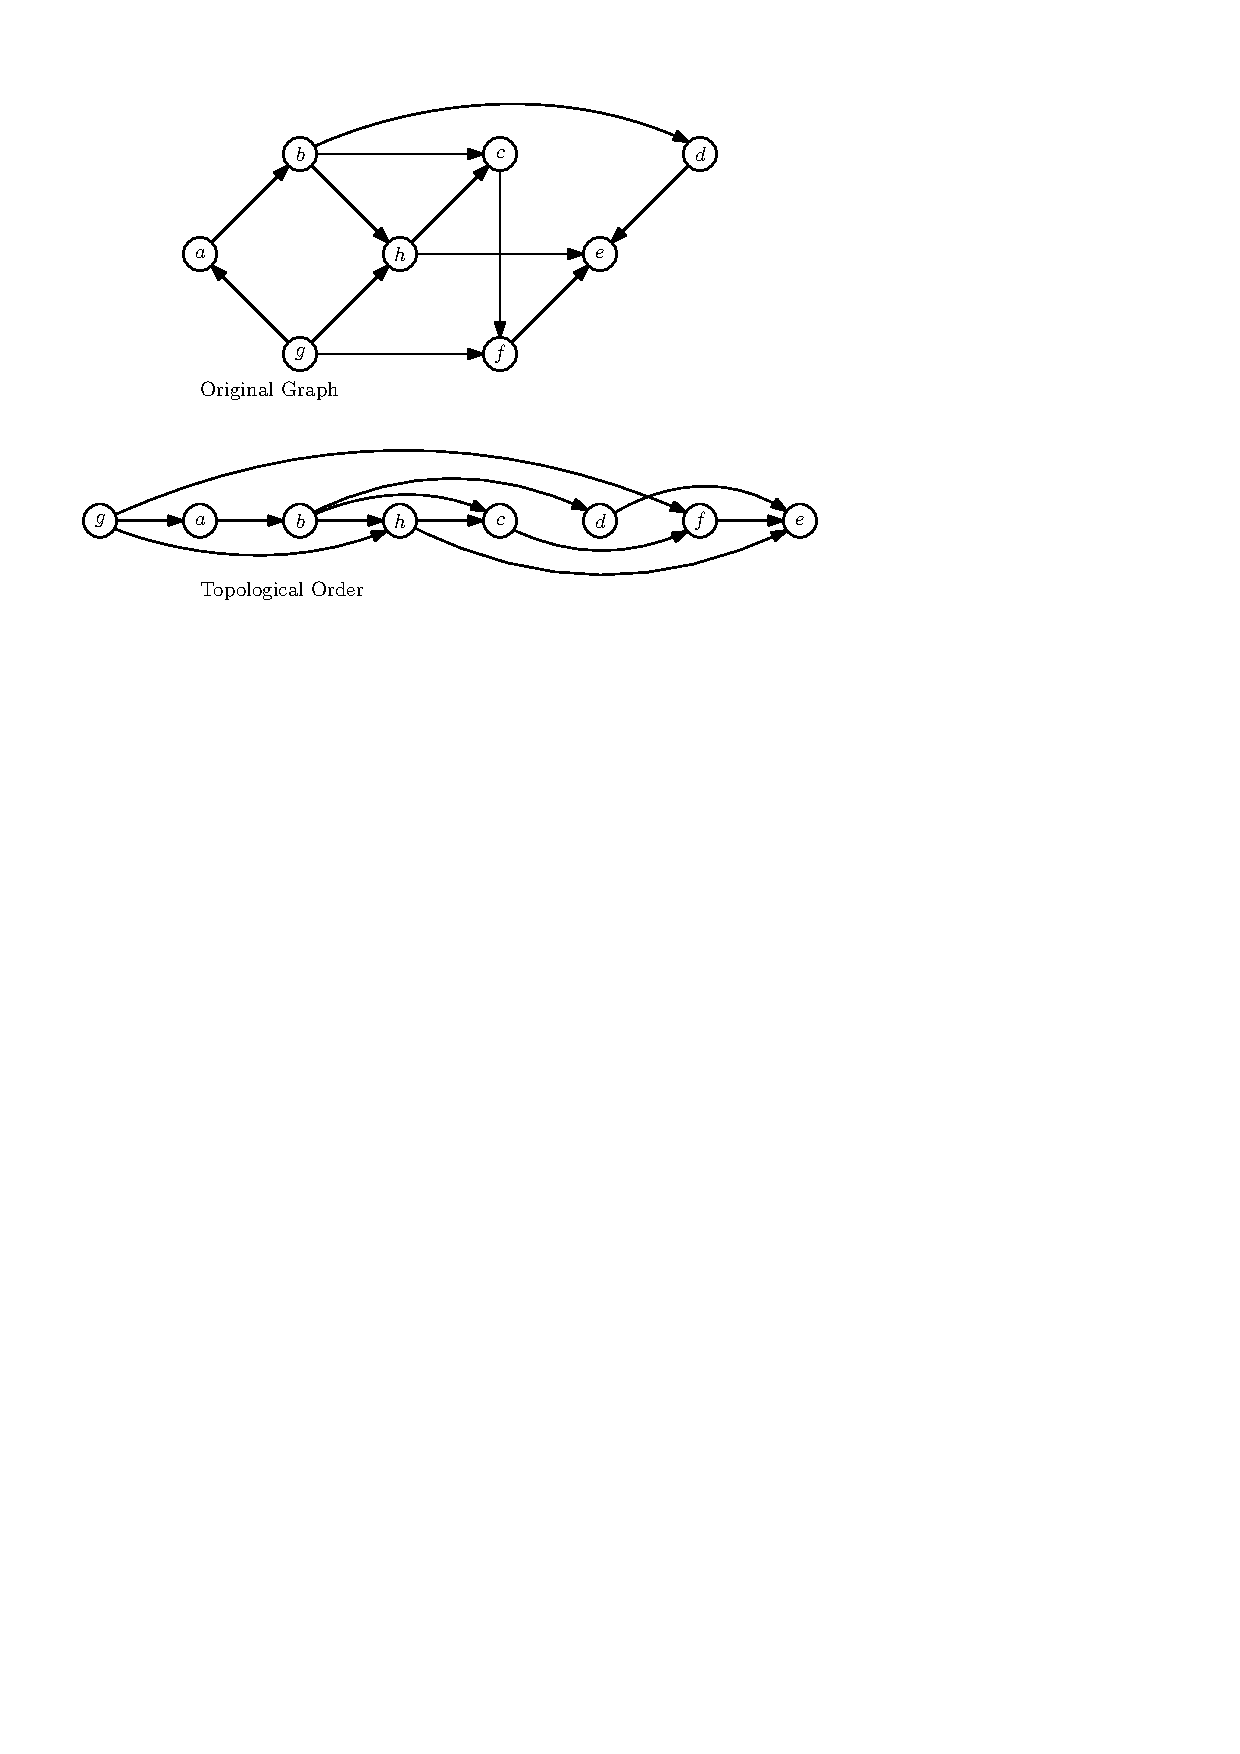
\includegraphics[width=.8\textwidth]{running2a}
    \end{figure}

    \begin{figure}[H]
        \caption{Topological Order for Second Graph}\label{2.b}
        \centering
        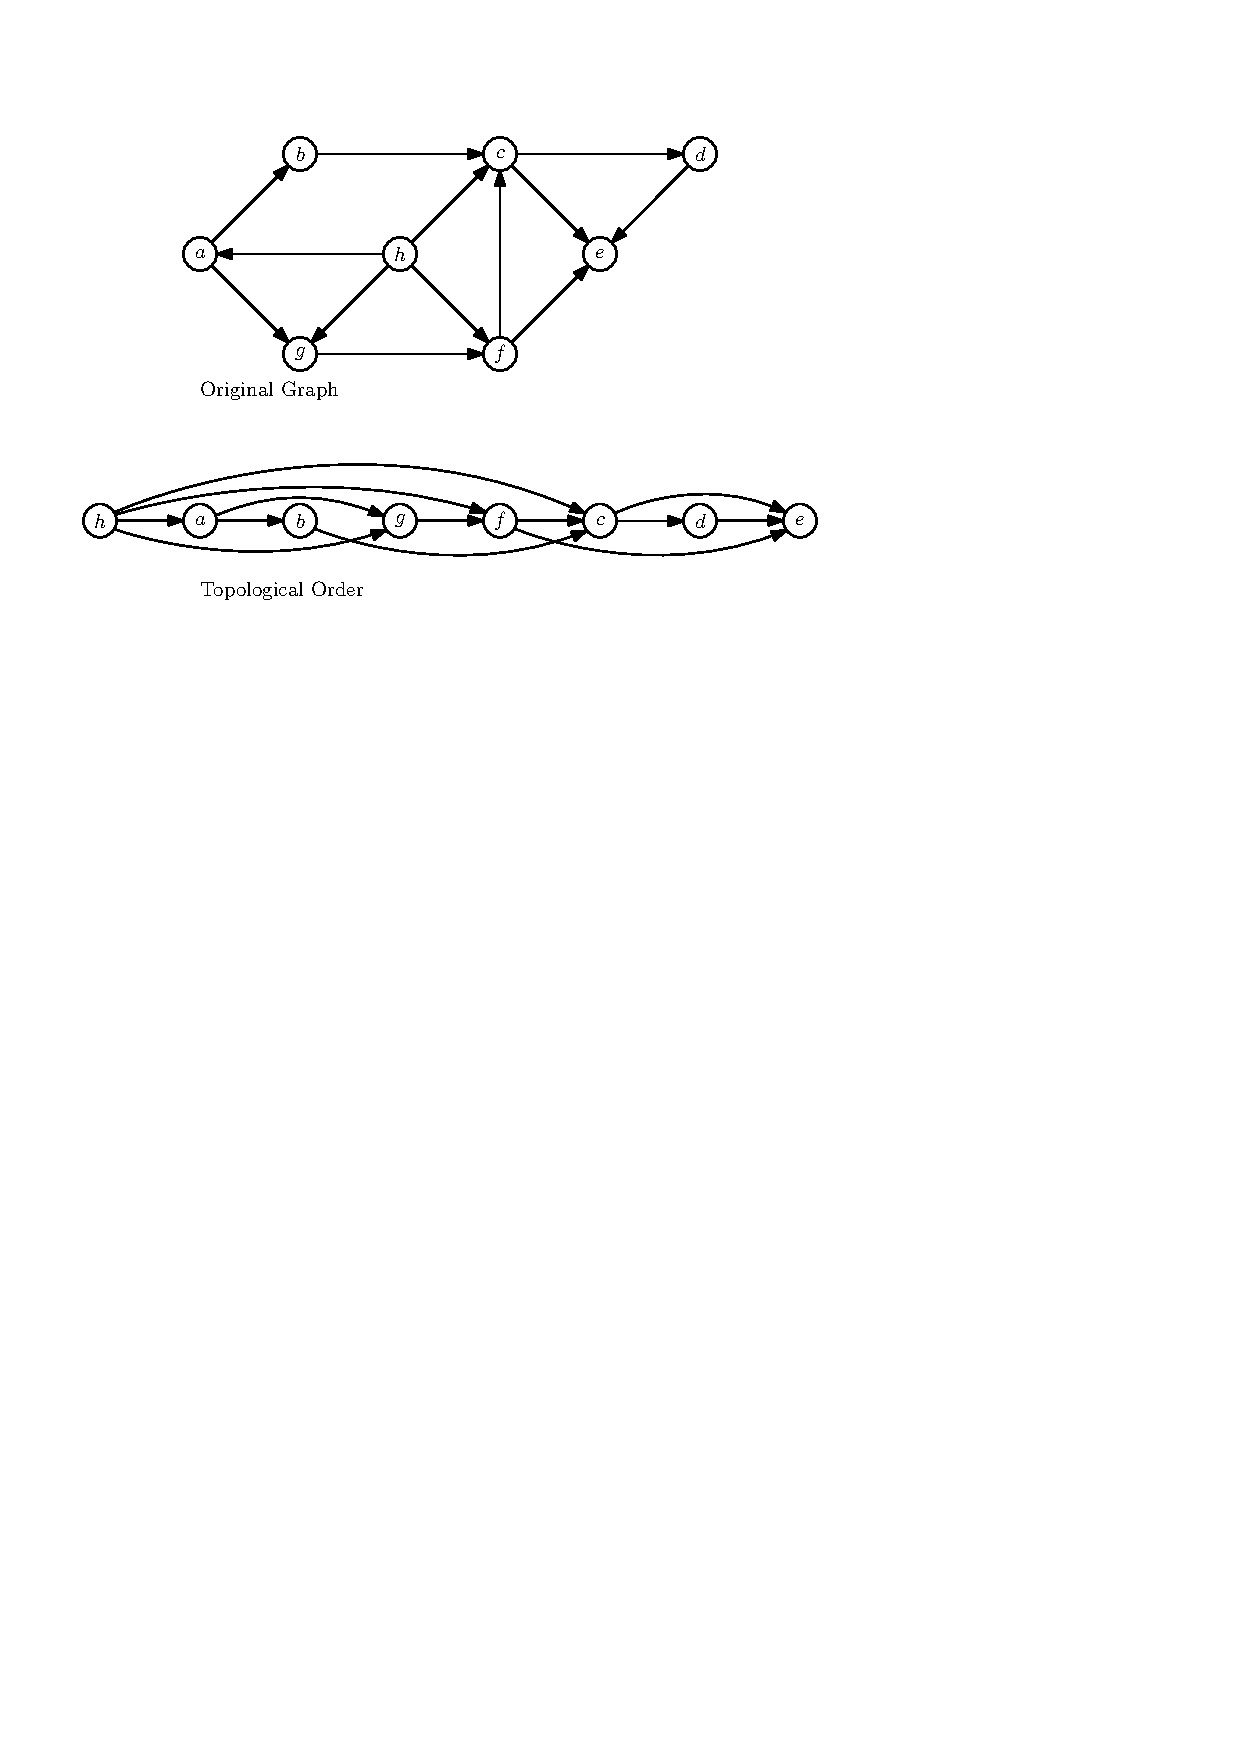
\includegraphics[width=.8\textwidth]{running2b}
    \end{figure}
\end{homeworkSubProblem}

\begin{homeworkSubProblem}
    The MST generation order is shown in \cref{3}, from which we know
    that the weight of the fifth edge added for graph 1 is $3$,
    for graph 2 is $7$.

    \begin{figure}[H]
        \caption{Prim's Algorithm Edge Added Order for First Graph}\label{3}
        \centering
        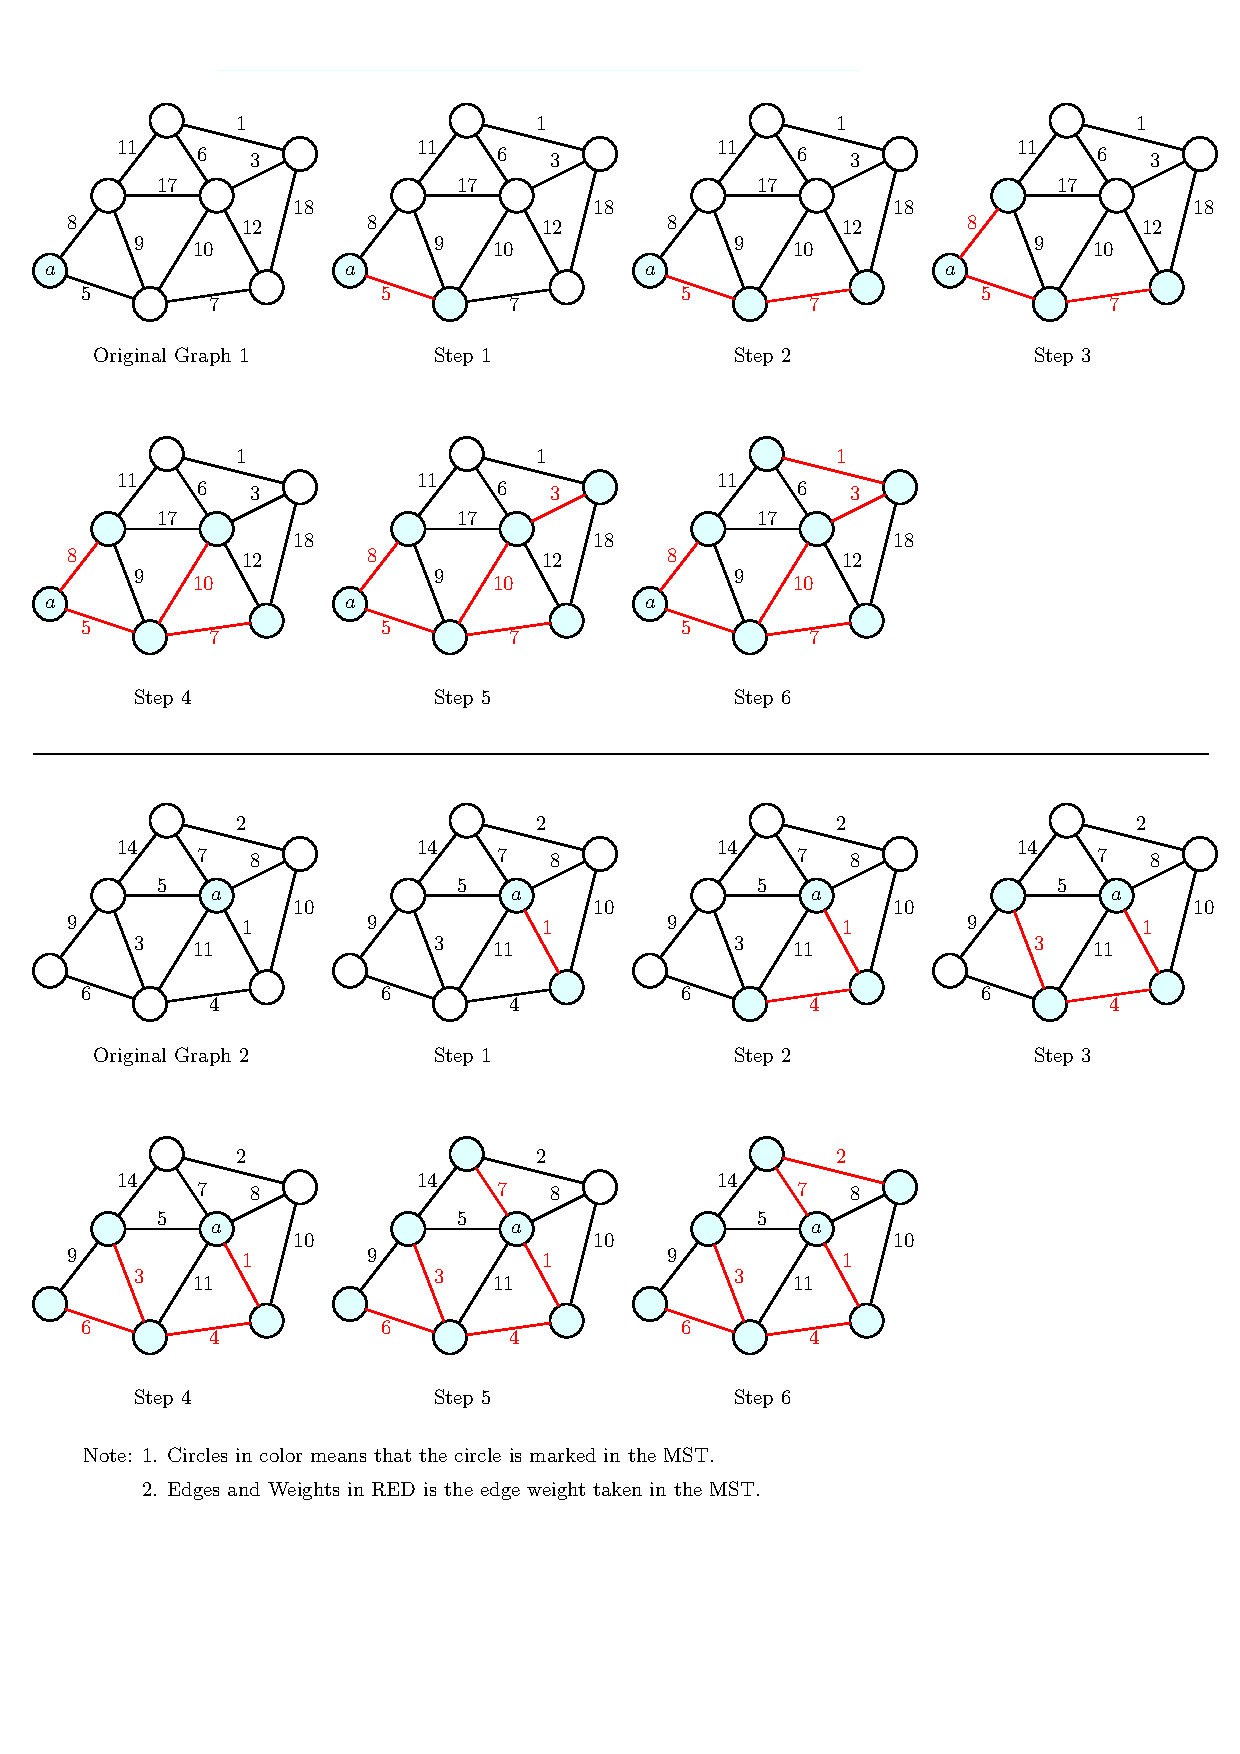
\includegraphics[width=\textwidth]{running3}
    \end{figure}
\end{homeworkSubProblem}

\begin{homeworkSubProblem}
s
    \begin{figure}[H]
        \caption{Prim's Algorithm Edge Added Order for First Graph}\label{4}
        \centering
        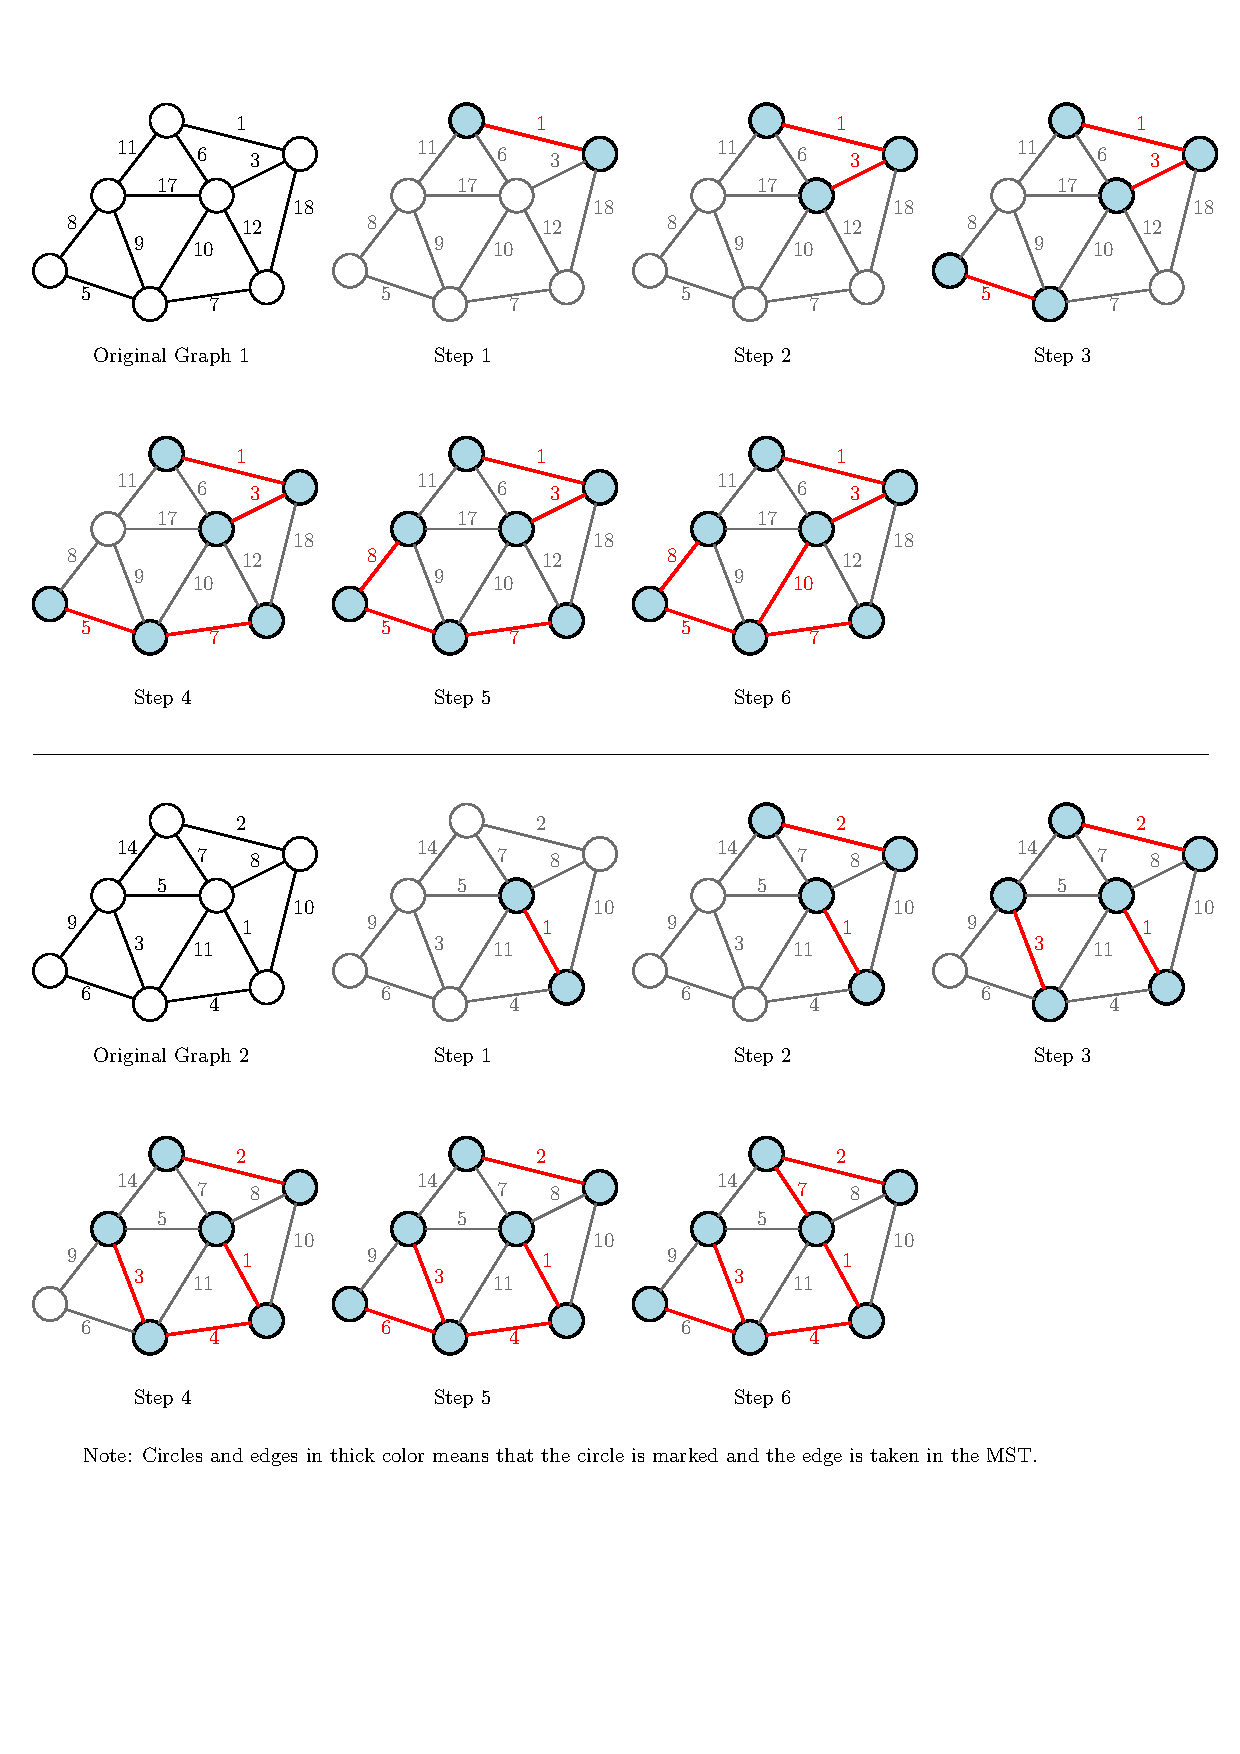
\includegraphics[width=\textwidth]{running4}
    \end{figure}
\end{homeworkSubProblem}
\end{homeworkProblem}


\begin{homeworkProblem}[Minimum Spanning Tree Problem]
to-do
\end{homeworkProblem}


\section*{TA's Feedback}
P4-c's algorithm has some mistake.
Final score: 99.

\end{document}
